\chapter{Manual de usuario}
\label{chap::manual}

\drop{E}{ste} apéndice pretende servir de guía o manual de usuario para BreakBrain. A lo largo del mismo se expondrán las diferentes páginas que componen la red social, para después explicar paso a paso cómo se deben desempeñar algunas de las tareas más comunes que un usuario puede necesitar realizar durante el uso de BreakBrain.

\section{Las páginas de BreakBrain}

\subsection{Inicio de sesión (login)}

Esta es la página de incio de sesión. Se trata de la página que se muestra al entrar en {\tt www.breakbrain.com}. Desde ella también es posible registrarse como usuario de la plataforma, desplegando el componente de registro.

\begin{figure}[h]
  \begin{center}
    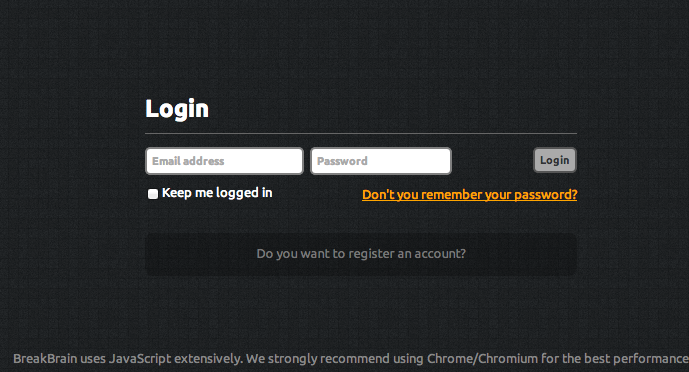
\includegraphics[width=\textwidth]{./images/page-login.png}
  \end{center}  
  \caption{Página de inicio de BreakBrain}
  \label{fig::page-login}
\end{figure}

\subsection{Página principal (home)}

Se trata de la página principal, a la que se accede directamente iniciando sesión. En ella se ofrece un resumen breve del estado del entrenamiento cerebral, así como algunas actualizaciones de otros usuarios y los juegos recomendados.

\begin{figure}[h]
  \begin{center}
    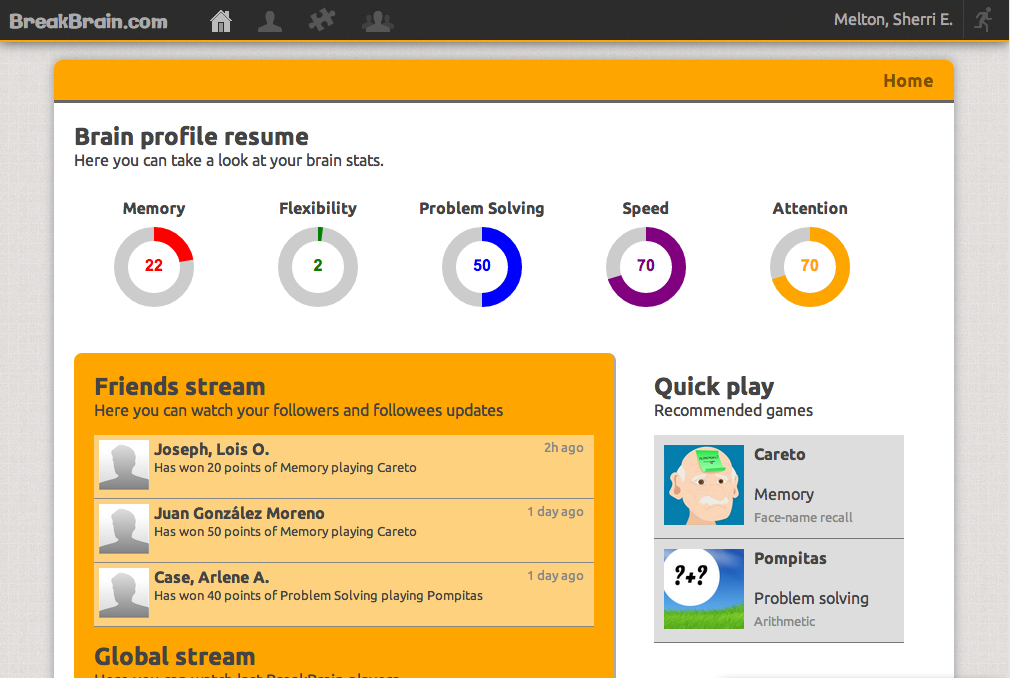
\includegraphics[width=\textwidth]{./images/page-home.png}
  \end{center}  
  \caption{Página principal de BreakBrain}
  \label{fig::page-home}
\end{figure}

\subsection{Perfil (profile)}

En esta página se muestra la información personal del usuario, la especificación de sus intereses de entrenamient, todas las estadísticas del mismo y sus métricas sociales: {\it followers} y {\it followees}.

Los campos de intereses e información personal son directamente editables.

\begin{figure}[h]
  \begin{center}
    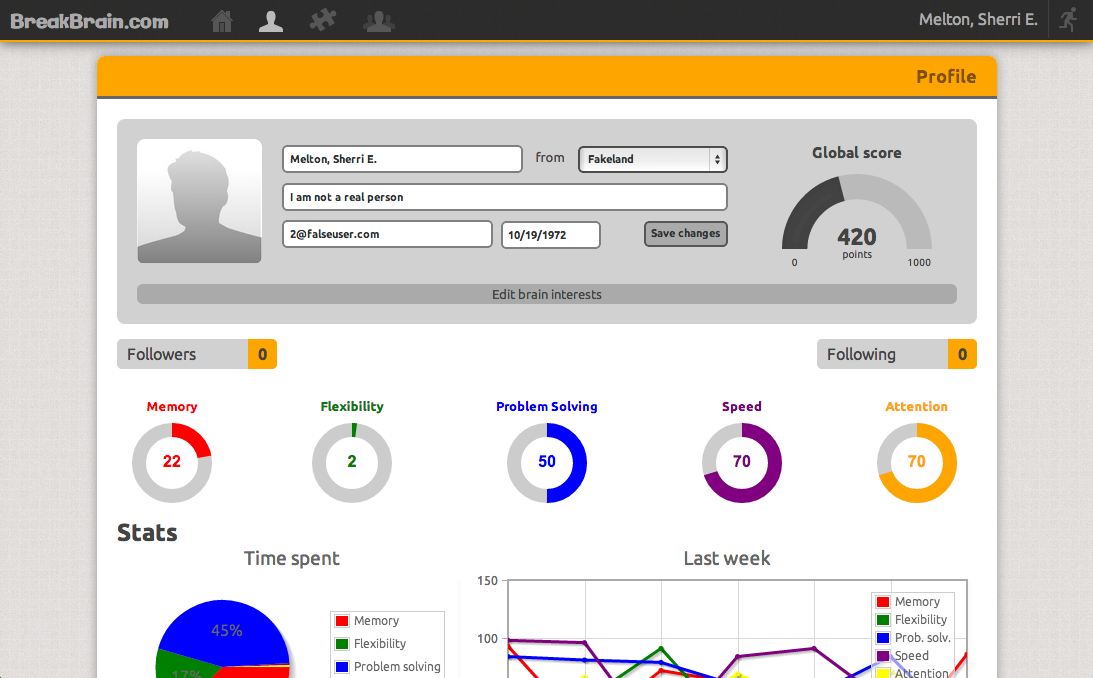
\includegraphics[width=\textwidth]{./images/page-profile.png}
  \end{center}  
  \caption{Perfil de usuario de BreakBrain}
  \label{fig::page-profile}
\end{figure}

\subsection{Juegos (games)}

La página de juegos de BreakBrain muestra todos los juegos disponibles, categorizados según la capacidad mental y habilidad a la que pertenecen. Haciendo click sobre un juego éste se carga y empieza la partida.

\begin{figure}[h]
  \begin{center}
    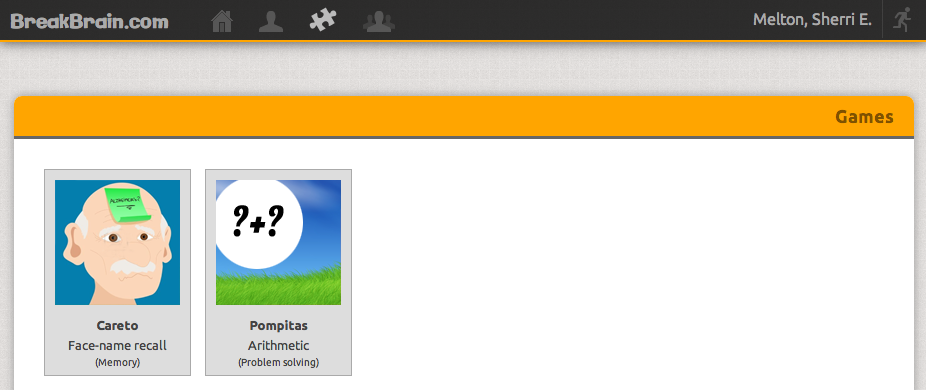
\includegraphics[width=\textwidth]{./images/page-games.png}
  \end{center}  
  \caption{Juegos de BreakBrain}
  \label{fig::page-games}
\end{figure}

\subsection{Gente (people)}

Esta página recomienda usuarios a los que seguir y permite realizar búsquedas basadas en nombre, nick y país. Haciendo click en cada resultado se carga la información completa del usuario seleccionado, permitiendo seguirlo o dejar de hacerlo (en caso de que ya se le esté siguiendo).

\begin{figure}[h]
  \begin{center}
    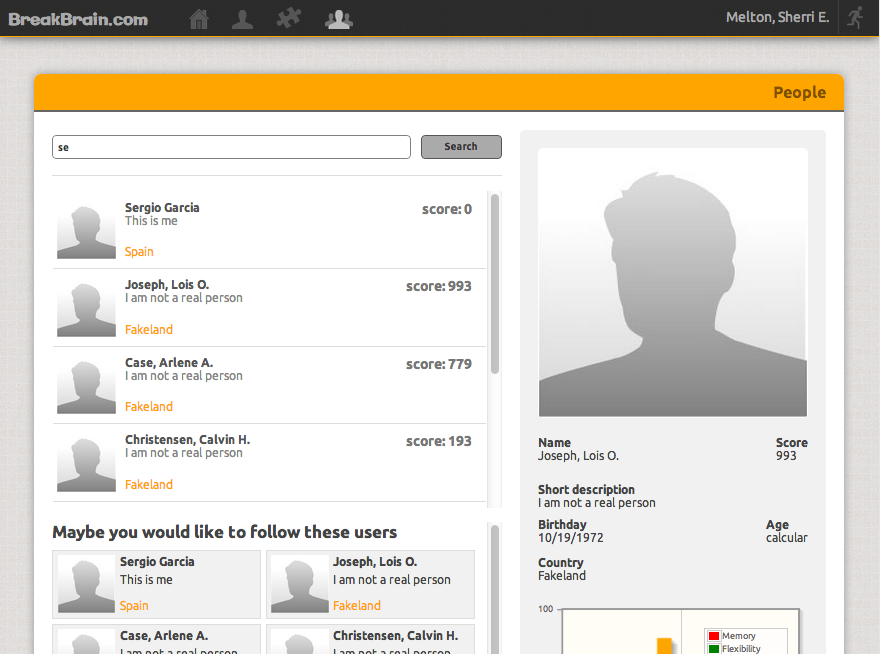
\includegraphics[width=\textwidth]{./images/page-people.png}
  \end{center}  
  \caption{Búsqueda y recomendación de personas en BreakBrain}
  \label{fig::page-people}
\end{figure}

\section{Tareas comunes}

A continuación se explican los pasos necesarios para llevar a cabo las tareas más comunes utilizando BreakBrain, como son el registro de un usuario, la recuperación de contraseña, la configuración del entrenamiento, etc.

\subsection{Creando una nueva cuenta de usuario}

Para crear una cuenta de usuario nueva de BreakBrain basta con acceder a la página de login {\tt /login.html} (figura \ref{fig::page-login}). Una vez cargada la página debemos desplegar el componente de registro y rellenar nuestros datos (ver figura \ref{fig::page-register}). En este paso es especialmente importante indicar bien nuestra dirección de e-mail, ya que BreakBrain nos enviará un correo de confirmación para que activemos la cuenta y podamos empezar a utilizarla.

\begin{figure}[h]
  \begin{center}
    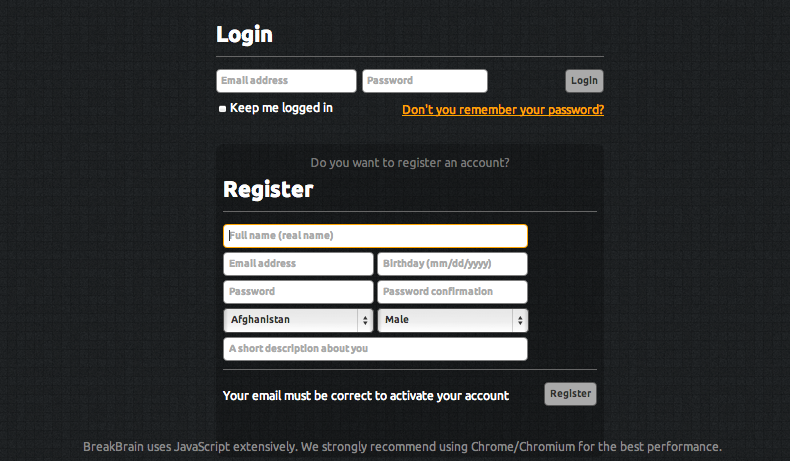
\includegraphics[width=\textwidth]{./images/page-register.png}
  \end{center}  
  \caption{Formulario de registro de BreakBrain}
  \label{fig::page-register}
\end{figure}

Una vez creemos nuestra cuenta, recibiremos un email de activación de la misma (figura \ref{fig::register-email}). Hasta que no la activemos no podremos empezar a utilizarla. La activación es sencilla, y basta con hacer click sobre el enlace que incluye el email. Después de hacerlo ya podremos hacer login con nuestra nueva cuenta.

\begin{figure}[h]
  \begin{center}
    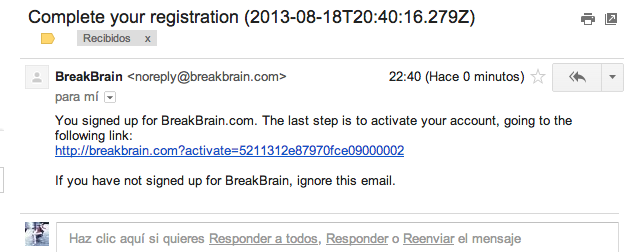
\includegraphics[width=\textwidth]{./images/register-email.png}
  \end{center}  
  \caption{Email de activación de cuenta de BreakBrain}
  \label{fig::register-email}
\end{figure}

\subsubsection{Recuperando la contraseña olvidada}

En caso de que olvidemos nuestra contraseña, BreakBrain nos permitirá crear una nueva mediante la dirección de email que indicamos en el proceso de registro. Para seguir este proceso basta con hacer click sobre el enlace de recuperación de contraseña de la página de login (figura \ref{fig::page-login}) y escribir la dirección de email que usamos en su día para realizar el registro.

\begin{figure}[h]
  \begin{center}
    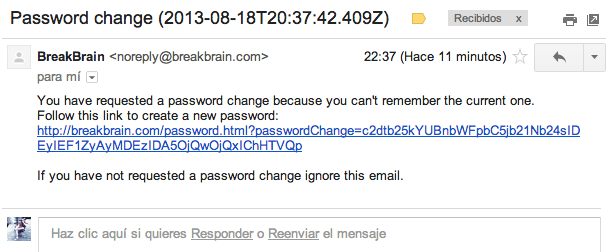
\includegraphics[width=\textwidth]{./images/password-change.png}
  \end{center}  
  \caption{Email de recuperación de contraseña de BreakBrain}
  \label{fig::recover-email}
\end{figure}

Recibiremos un email de recuperación de contraseña (figura \ref{fig::recover-email}). Haciendo click sobre el enlace que incluye accederemos a una página en la que escribir nuestra nueva contraseña (figura \ref{fig::recover-pass}). Rellenarla y confirmar será suficiente para que podamos volver a utilizar BreakBrain, con la nueva contraseña, eso sí.

\begin{figure}[h]
  \begin{center}
    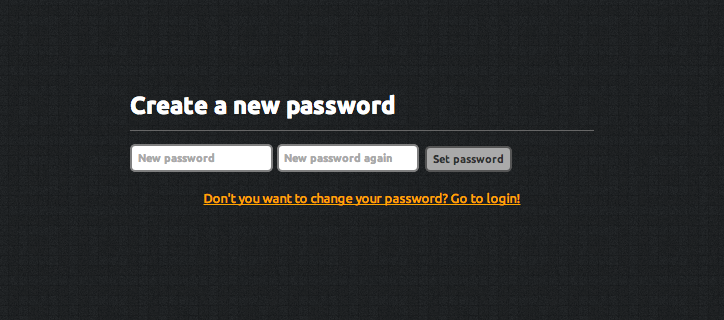
\includegraphics[width=\textwidth]{./images/page-password.png}
  \end{center}  
  \caption{Página de recuperación de contraseña de BreakBrain}
  \label{fig::recover-pass}
\end{figure}

\subsection{Completando el perfil de usuario}

La página de perfil de usuario (figura \ref{fig::page-profile}), además de mostrar toda nuestra información personal y estadísticas de progresión del entrenamiento, permite editar cualquier campo directamente. El botón {\it ``save changes''} guardará cualquier cambio que hayamos hecho.

\subsubsection{Definiendo las preferencias de entrenamiento}

En la página de perfil, bajo nuestra información personal, se encuentra un desplegable de configuración donde podemos elegir en qué habilidades mentales queremos centrar nuestro entrenamiento con BreakBrain.

\begin{figure}[h]
  \begin{center}
    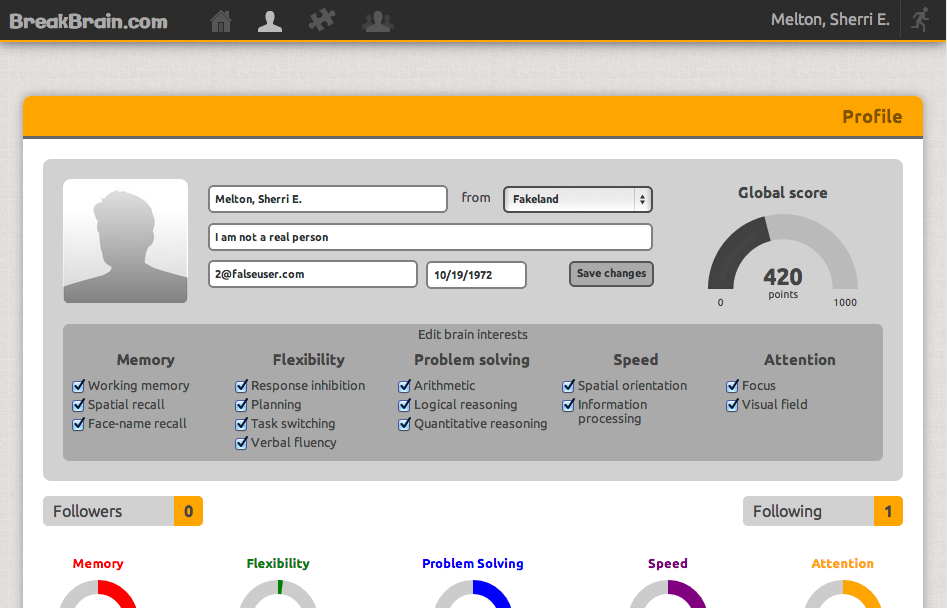
\includegraphics[width=\textwidth]{./images/training-settings.png}
  \end{center}  
  \caption{Configuración de entrenamiento cerebral}
  \label{fig::training-settings}
\end{figure}

La figura \ref{fig::training-settings} muestra el componente de configuración de entrenamiento una vez desplegado. Únicamente se tendrán en cuenta para el cálculo de nuestro progreso y recomendación de usuarios y juegos los intereses marcados. No obstante, es posible modificar la configuración de entrenamiento en cualquier momento.

\subsection{Siguiendo a otros usuarios}

La suscripción a novedades de otros usuarios, lo que en BreakBrain se denomina {\it seguir} a usuarios, es realmente sencilla. En la página de búsqueda de gente (figura \ref{fig::page-people}), cuando hacemos click sobre un resultado de búsqueda o recomendación para mostrar el perfil completo, aparece un botón para seguir al usuario (o dejar de hacerlo, si ya lo estamos siguiendo). La figura \ref{fig::follow-button} muestra dicho botón.

\begin{figure}[h]
  \begin{center}
    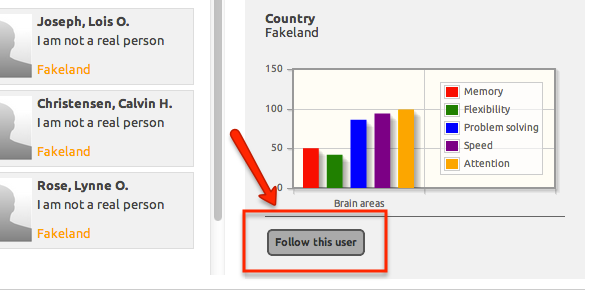
\includegraphics[width=\textwidth]{./images/follow-button.png}
  \end{center}  
  \caption{Botón de seguimiento de usuarios}
  \label{fig::follow-button}
\end{figure}

\subsection{Entrenando el cerebro con juegos}

\subsubsection{Juegos monojugador}

\subsubsection{Jugando contra otros usuarios}
